\chapter{Background}
	\label{chap:background}
	
	This chapter gives an overview of the work being done on brain simulators. It
	begins with a history of the models used to simulate the brain which led to
	the current generation of `spiking neural networks' and the computational
	challenges these bring. The latest super-computer technology is then presented
	with an explanation of its unsuitability for neural simulation. This is
	followed by a discussion of the various attempts made to produce a
	special-purpose architecture for this task looking in particular at the highly
	flexible SpiNNaker architecture. The chapter concludes by examining the
	technology used in SpiNNaker and other super-computers to allow fast
	communication within these systems.
	
	\section{Simulating Brains}
		
		\label{sec:simulating-brains}
		
		Efforts to simulate the brain focus on building approximate but
		representative models of its behaviour. Most current brain models attempt to
		capture the way that neurons behave and communicate with each other.
		Typically, the network is expressed as a graph of neurons which take inputs
		from other neurons and perform some simple computation to produce an output
		which is, in turn, connected to other neurons. This type of model is known
		generally as an Artificial Neural Network (ANN).
		
		\subsection{Generations of ANN}
			
			The development of ANNs can be divided up into three coarse generations,
			each increasing their level of biological realism \cite{vainbrand11}.
			
			The first generation of ANNs, such as the McCulloch-Pitts threshold neuron
			\cite{mcculloch43}, consisted of testing if a simple, linear function of
			the neuron's inputs was above a threshold value and outputting either a
			`high' or `low' signal. The function used in each neuron and the pattern
			of connectivity in the network define the behaviour of the network as a
			whole.
			
			It was realised that communication between neurons is not level-based but
			instead appears to be based on the rate at which `spikes' are produced (or
			`fired') by neurons to their neighbours. The second generation of ANNs
			seek to model this by representing the `firing rate' as their output in a
			continuous value \cite{maass97}. Once again, the network's behaviour was
			defined by the functions computed by each neuron and the network's
			connectivity.
			
			The third generation of ANNs extends the idea further by realising that
			the firing rate is not the only significant factor but the timing of the
			arrival of spikes is too \cite{maass01}. Typically these Spiking Neural
			Networks (SNNs) work on the principle related to the `leaky integrate and
			fire' model. Here each spike either positively or negatively contributes
			to the amount of `charge' stored in the neuron (that is, the charge is
			integrated over time). Once the charge reaches a certain threshold, the
			neuron `fires' causing a spike to be transmitted and the charge in the
			neuron to return to zero. Charge in the neuron also constantly `leaks'
			away such that if the neuron doesn't receive any spikes its charge will
			eventually return to 0. This process is illustrated in figure
			\ref{fig:snn-example}
			
			\begin{figure}
				\center
				\input{|"python2 figures/snn-example.py"}
				\caption{Simple leaky-intergrate-and-fire neuron example.}
				\label{fig:snn-example}
			\end{figure}
		
		\subsection{Computational Challenges}
			
			Simulating ANNs, and in particular SNNs, presents a number of
			computational challenges.
			
			The first issue is that real, biological neural networks can contain
			billions of neurons. An adult human, for example, has around 85 billion
			neurons \cite{herculano09}. As a result, the size of biological-scale
			networks can be extremely large requiring vast amounts of conventional
			computational resource to model. Conventionally this is achieved using
			large, parallel computers.
			
			The second issue is that each neuron is typically connected to thousands
			of others. As a result of this, huge amounts of one-to-many communication
			must take place between the processing nodes simulating the neurons.  By
			contrast, conventional electronic circuits, and consequently conventional
			computing systems, tend to feature one-to-one and one-to-few connections
			as the power needed to send a signal to many places at once can be large.
			
			Luckily most communication occurring in the brain is highly local which
			means that spikes do not usually need to be transmitted to neurons far
			away. Neurons also tend to fire at a relatively slow rate compared to
			electronic components with firing rates being measured in terms of hertz
			while modern electronics operates at multiple gigahertz. As a result
			time-division multiplexing can be used in order to use a single processing
			node or communication channel for many different neurons and spikes at
			once respectively.
	
	
	\section{Super-Computers}
		
		\label{sec:super-computers}
		
		\begin{table}
			\center
			\begin{tabular}{r l r r r l l l}
				\toprule
				Rank & Name    & Pflops& Cores  & Nodes  & Topology & Interconnect          & Sources \\
				\midrule                          
				1 & Tianhe-2   & 33.86 & 3,120,000 & 16,000 & Fat-Tree & Electrical \& Optical & \cite{dongarra13} \\
				2 & Titan      & 17.59 & 560,640   & 18,688 & 3D Torus & Electrical            & \cite{bland12} \\
				3 & Sequoia    & 17.17 & 1,572,864 & 98,304 & 5D Torus & Electrical \& Optical & \cite{prickett10} \\
				4 & K Computer & 10.51 & 705,024   & 68,544 & 6D Torus & Electrical            & \cite{fujitsu11,yokokawa11} \\
				5 & Mira       &  8.59 & 786,432   & 49,152 & 5D Torus & Electrical \& Optical & \cite{prickett10} \\
				\bottomrule
			\end{tabular}
			
			\caption{Top Five `Top500' Super-Computers, November 2013 \cite{meuer13n}.}
			\label{tab:top500}
		\end{table}
		
		The Top500 list \cite{meuer13n} aims to enumerate biannually the 500 fastest
		super-computers ranked by their performance on the LINPACK benchmark
		\cite{dongarraLINPAC}. The list offers an insight into the current
		state-of-the-art for high-performance computing. Table \ref{tab:top500}
		shows the top five machines in the Top500 list released in November 2013
		along with basic details of the type of interconnection involved. In this
		section an overview is given of the architecture of these large scale
		machines.
		
		The LINPACK benchmark performs computations to ``analyze and solve linear
		equations and linear least-squares problems'' to produce a computational
		load representative of certain computational tasks common to scientific
		computing \cite{dongarra84}. In particular it is a CPU-bound problem which
		attempts to measure the peak CPU performance achievable\footnote{Where CPU
		Performance is measured in Petaflops: how many quadrillion ($10^{15}$)
		floating point operations can be performed per second.} but without any
		significant indication of the performance of the network which connects the
		system together \cite{dongarra07}.
		
		Since simulation of SNNs requires a large amount of communication but
		relatively small amounts of computation, this benchmark is not
		representative of the workload of such a task. Despite the shortcomings of
		the LINPACK benchmark there is unsurprisingly a high degree of correlation
		between CPU power and interconnect performance in the best Top500 machines.
		The Graph500 list is a more recent, complementary ranking which uses
		benchmarks based on graph traversal problems \cite{murphy10}. Such problems
		rely on having efficient point-to-point communication between different
		parts of the system where each section of the graph resides. With the
		exception of Titan, which was not measured, the top five Top500 computers
		also sit within the top six places of Graph500 \cite{murphy13n}. As a
		result, due to its maturity and wider scope, the Top500 list is discussed in
		this section.
		
		\subsection{Anatomy of a Super-Computer}
			
			Large computer systems are typically built by combining a large number of
			`processing elements' in such a way that they are able to communicate
			efficiently. These processing elements come in many forms though the three
			most prevalent:
			
			\begin{description}
				
				\item[General Purpose Processor] A conventional processor `core' as
				found in desktop and mobile computer CPUs. These flexible devices have
				historically represented the vast majority of the Top500's computing
				power.
				
				\item[Graphics Processing Unit (GPU)] A specialised processor which is
				able to efficiently perform the same operation across a large number of
				data elements simultaneously. The Titan super-computer notably makes
				extensive use of GPUs \cite{bland12}.
				
				\item[Accelerators] Increasingly other forms of compute resource, such
				as the Intel Xeon Phi accelerator in Tianhe-2 are being used. The Xeon
				Phi contains 57 medium-sized general purpose cores which can be used to
				complement a conventional multi-core system \cite{dongarra13}.
				
			\end{description}
			
			A number of these individual processor cores are then combined together to
			create a single `node' in the system. Typically the cores within a node
			are able to communicate relatively cheaply while messages to remote nodes
			must traverse a slower system-wide interconnection network.
		
		\subsection{Topology}
			
			The topology of the system-wide interconnect has a great influence on the
			performance of a super-computer. Typically the topology of these networks
			is such that communication between near-by nodes is cheap and does not
			compete with distant nodes for communication resources. The top five
			machines in the Top500 list achieve this using the `fat tree' and `torus'
			topologies described below.
			
			\subsubsection{Fat Trees}
				
				\begin{figure}
					\begin{subfigure}[t]{\textwidth}
						\center
						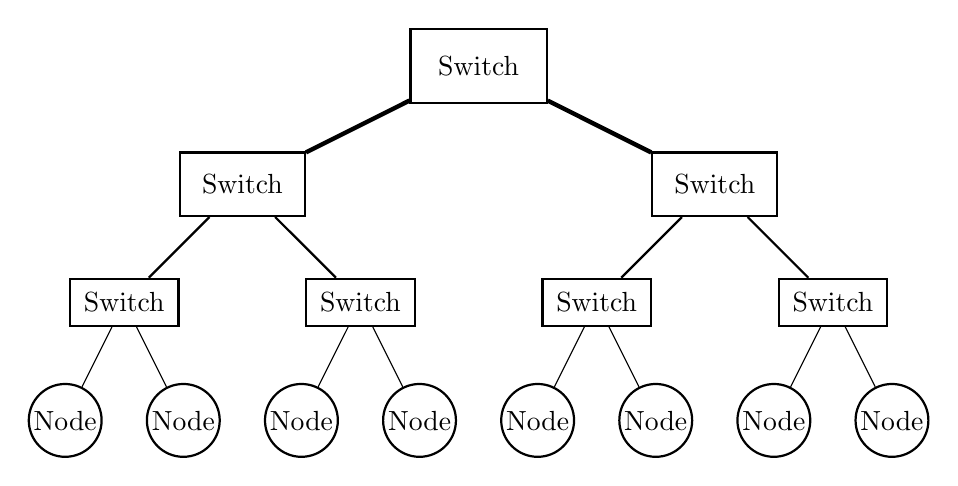
\begin{tikzpicture}[thick, node distance=1em]
	
	\begin{scope}[every node/.style={draw,rectangle,thick},inner sep=1.0em]
		\tikzstyle{level 1}=[sibling distance=6cm,every child/.style={ultra thick},inner sep=0.8em]
		\tikzstyle{level 2}=[sibling distance=3cm,every child/.style={thick},inner sep=0.5em]
		\tikzstyle{level 3}=[sibling distance=1.5cm,every child/.style={thin},inner sep=0.1em]
		
		\node {Switch}
			child {node {Switch}
				child {node {Switch}
					child {node [circle] {Node}}
					child {node [circle] {Node}}
				}
				child {node {Switch}
					child {node [circle] {Node}}
					child {node [circle] {Node}}
				}
			}
			child {node {Switch}
				child {node {Switch}
					child {node [circle] {Node}}
					child {node [circle] {Node}}
				}
				child {node {Switch}
					child {node [circle] {Node}}
					child {node [circle] {Node}}
				}
			}
		;
	\end{scope}
	
\end{tikzpicture}

						\caption{Basic fat tree links.}
						\label{fig:fat-tree-concept}
					\end{subfigure}
					
					\vspace{1.5em}
					
					\begin{subfigure}[t]{\textwidth}
						\center
						\input{figures/fat-tree-closs}
						\caption{Folded Clos network.}
						\label{fig:fat-tree-closs}
					\end{subfigure}
					
					\caption[Fat tree topologies.]{Fat tree topologies. Thicker lines
					represent higher bandwidth links.}
					\label{fig:fat-tree}
				\end{figure}
			
				In a basic fat tree, nodes are connected in a tree structure to switches
				which in turn are connected to further levels of switches (figure
				\ref{fig:fat-tree-concept}). Connections higher in the switch hierarchy
				are connected via links of increasing bandwidth to avoid the bandwidth
				bottle-neck around the root node. For a node to communicate, it
				sends its message to its parent switch which forwards the packet through
				the tree to its destination.
				
				In practice, such as in large machines like `Tianhe-2', it is not
				possible to build a switch with the required bandwidth of the higher
				nodes of a fat tree. In addition, the root switch is a potential single
				point of failure for the whole system. As a result, folded Clos networks
				are often used instead and have become synonymous with the fat tree
				topology. As shown in figure \ref{fig:fat-tree-closs}, traffic is split
				between two top-level switches reducing the bandwidth requirement for
				each. In addition, if a top-level switch fails messages can simply be
				routed using the other switch.
				
				Fat trees give small maximum hop-counts ($O(\log{N})$ with respect to
				the number of nodes in the system) to send a message from one node to
				any other. They also allow near-by nodes to communicate in a small
				number of hops. Unfortunately, such topologies depend on high-radix
				switches which can connect many nodes simultaneously.  Tianhe-2, for
				example, has thirteen 576-port switches based on a custom router chip.
				The cost of using high-radix switches is typically that of increased
				latency. In the case of Tianhe-2, the latency of a message broadcast to
				all nodes in the system is around 9$\mu$s or about 19,800
				CPU\footnote{Intel Ivy Bridge CPUs running at 2.2 GHz} cycles
				\cite{dongarra13}.
				
				To allow multiple simultaneous computation tasks to share the
				super-computer's resources, fat trees can be trivially partitioned by
				allocating whole sub-trees to a given task.
			
			\subsubsection{Tori}
				
				\begin{figure}
					\begin{subfigure}[t]{\textwidth}
						\center
						\input{figures/torus-flat}
						\caption{Mesh (Grey lines show wrap-around connections added in a
						torus)}
						\label{fig:torus-flat}
					\end{subfigure}
					
					\vspace{1em}
					
					\begin{subfigure}[t]{\textwidth}
						\center
						\input{figures/torus-pipe}
						\caption{Rolled into a tube}
						\label{fig:torus-pipe}
					\end{subfigure}
					
					\vspace{1em}
					
					\begin{subfigure}[t]{\textwidth}
						\center
						\input{figures/torus-3D}
						\caption{Bent into a torus}
						\label{fig:torus-3D}
					\end{subfigure}
					
					\caption{Transformation of a mesh into a torus.}
					\label{fig:forming-a-torus}
				\end{figure}
			
				The most common topology which features in all but one of the top-five
				is the torus (also known as a $k$-ary $n$-cube). In this topology, nodes
				are arranged in a $n$-dimensional mesh. Nodes at the extreme edges of
				the mesh are connected together to form a torus. In the 2D case this can
				be visualised as in figure \ref{fig:forming-a-torus}. Starting with a
				regular 2D mesh (figure \ref{fig:torus-flat}), the top- and bottom-most
				nodes are connected together to form a tube (figure
				\ref{fig:torus-pipe}).  Then the left- and right-most nodes of the tube
				are connected together forming a torus (figure \ref{fig:torus-3D}).
				Though harder to visualise, this process generalises to toruses of
				higher dimensions.
				
				Each node is able to communicate directly with its immediate neighbours
				in each dimension, that is above, below, left and right in the 2D case.
				More distant nodes are able to communicate by forwarding messages via
				intermediate nodes.
				
				Because nodes in a torus only communicate directly with their
				neighbours, the switches required in each node may be of a low radix
				compared to those in the fat tree. For an $n$-dimensional torus, each
				node requires a radix $2n+1$ switches independent of the total number of
				nodes in the system.
				
				Compared with a fat tree, however, a greater number of hops is required
				in the worst case where two nodes are distant. In a torus $k$ nodes long
				in each of $n$ dimensions the worst case path length is $\frac{kn}{2}$
				\cite{dally04}. As a result, though the individual hops are less
				expensive, the time taken to broadcast a message to all nodes in a large
				Blue Gene/Q supercomputer such as Sequoia is 17 $\mu$s compared to 9
				$\mu$s for the same operation in Tianhe-2 \cite{morozov12}.
				
				Higher dimensional tori are also easily partitioned into a number of
				lower-dimensional tori or meshes to allow machines to be shared between
				many independent computing tasks \cite{yokokawa11,chen11}.
		
		\subsection{Interconnect}
			
			The physical links responsible for connecting machines are another
			important factor in the performance achievable by a given interconnection
			system. The current state-of-the-art techniques fall into two categories:
			electrical (`high-speed serial') and optical transmission.
			
			Electrical transmission technologies are generally much cheaper than
			optical for short distances and lower bandwidths. As a result connections
			between physically neighbouring nodes are almost universally connected via
			such links. In systems such as Blue Gene/Q and Tianhe-2 optical links are
			used to connect between different cabinets in the system
			\cite{dongarra13,prickett10}. These optical links are able to carry the
			equivalent of many electrical signals over longer distances at the expense
			of more complex hardware requirements for transmitters and receivers.
			
			The topology of a network can greatly influence the difficulty of
			physically connecting nodes arranged in cabinets. The use of cabinets
			essentially map the physical nodes into an approximately 2D sheet. As a
			result, for torus networks of more than two dimensions, links which are
			physically short in higher dimensions can result in long wires between
			distant cabinets. For hierarchical networks such as fat trees, long wires
			arise from the need to connect together distant parts of a system at the
			higher levels of the hierarchy. Long wires are both more difficult to
			install and require more expensive link technologies. The preliminary work
			described in \S\ref{sec:wiring-up-large-spinnaker-machines} explores these
			issues in further detail.
	
	\section{Hardware Neural Simulators}
		
		Current super-computers are heavily focused on computation-heavy tasks as is
		apparent from the use of hundreds of thousands of high-end processor cores
		in the Top500's top five machines. The Blue Brain project \cite{markram06}
		makes use of such computationally powerful machines to simulate relatively
		small ANNs of tens of thousands of realistic neurons. Large ANNs using the
		less realistic models of neuron behaviour change the balance between
		computation and communication.  Requiring relatively little computation for
		each neuron but needing vast amounts of communication, conventional super
		computers are a poor fit and, as a result, alternative architectures have
		been developed for neural simulation.
		
		\subsection{Electrical Technology}
		
			There are three distinct approaches being taken to designing (electrical)
			hardware for neural simulation. One is to use analogue electronic components
			for the entire system, another is to mix analogue and digital components and
			a final approach is to use traditional digital components. These three
			approaches and their merits are described below.
			
			\subsubsection{Analogue}
			
				Though analogue technology has long been out of favour for general
				purpose computing, it has been suggested for neural simulation as it is
				ultimately designed to model an analogue system: the brain. Neural
				models are highly fault-tolerant and do not assume that values will be
				calculated or communicated precisely. Modern digital computers, by
				contrast, have rigid requirements for the precision of values and so
				dedicate vast amounts of hardware and energy to guaranteeing precision,
				which is unnecessary in this case, making analogue simulators an
				attractive approach.
				
				A wide range of techniques for implementing the required functions in
				analogue circuitry has been proposed
				\cite{graf86,holler89,agranat90,azghadi13}. The analogue circuits used
				are often simple and replace more power-hungry general purpose
				processors \cite{misra10}. Even though the lack of precision of analogue
				circuits is not a problem for neural simulation, the lack of consistency
				is. The same analogue circuit may have widely different characteristics
				in one part of the chip compared to another due to variations in the
				silicon wafer. In addition circuits must tolerate changes in temperature
				and voltage, a task which is substantially more challenging for analogue
				circuits compared to their digital counterparts. As a result, current
				successful implementations such as the MIT Silicon Synapse have been
				limited to small parts of a neural network, a single synapse connecting
				two neurons in this case \cite{rachmuth11}.
				
				Finally, analogue systems make assumptions about the type of neural models
				that will be simulated limiting them to simulating only a handful of
				similar models. As a result, the current generation of analogue
				simulators lag behind the state-of-the-art in terms of ease-of-use and
				flexibility.
			
			\subsubsection{Mixed Mode}
				
				So-called `mixed mode' systems have been designed such as Neurogrid and
				BrainScaleS which combine analogue computational components with digital
				communication \cite{choudhary12,maguire07}. The use of digital
				communication avoids issues with inconsistencies across the chip while
				also simplifying routing of spikes which can then be completed using
				conventional digital methods.
				
				While offering improvements over purely analogue systems, many of the same
				drawbacks with variability and flexibility still apply.
			
			\subsubsection{Digital}
				
				Various groups have developed custom, digital, on-chip neural simulators
				\cite{prange93,jahnke96,schoenauer99,mehrtash03}. While successful in
				allowing relatively large numbers of neurons to be simulated, around 1
				million in the case of SP$^2$INN, along with the analogue and mixed mode
				designs above, these approaches are fundamentally restricted to only the
				models the designers originally intended \cite{mehrtash03}. Due to the
				lack of flexibility and increasing costs of designing custom silicon,
				researchers, such as those behind SP$^2$INN, have moved away from this
				approach.
				
				FPGAs (Field Programmable Gate Arrays) are, essentially, chips which can
				be electrically reprogrammed with custom logic circuits. They are now
				widely used in place of custom chips for performance-sensitive, highly
				specialised tasks as well as prototyping and development of conventional
				chips. Work using FPGAs to simulate neural models such as
				\cite{hellmich05} has allowed around half a million neurons with realistic
				numbers of connections between them to be simulated. Despite being
				considerably cheaper and far more flexible than completely custom
				hardware, FPGA development is still much slower than developing for
				general purpose CPUs and so still yields relatively inflexible systems.
				
				Finally, architectures based on general purpose digital processors are
				able to provide a great degree of flexibility at the expense of greater
				overhead\cite{furber07}. The SpiNNaker project, described in detail in the
				next section, has developed an architecture which combines many low-power
				processors which run neural simulations in software.
		
		\subsection{Topologies}
			
			Though various topologies have been used in hardware neural simulators
			these largely boil down to those based on to tori and trees. Unlike those
			in super-computers, the granularity of these networks tends to be higher
			reflecting the increased focus on communication over computation.  This
			subsection examines the topologies of two leading mixed-mode neural
			simulators, Neurogrid and BrainScaleS.
			
			\subsubsection{Neurogrid}
				
				The largest prototype Neurogrid system is able to support around 1
				million neurons in biological real-time using 100,000 times less power
				than a conventional super-computer. Its architecture, at the highest
				level, consists of a small number of Neurogrid chips  (16 in current
				prototypes) arranged as leaves in a binary-tree where spike events are
				routed to other chips \cite{choudhary12}.
				
				\begin{figure}
					\center
					\input{figures/neurogrid-chip}
					\caption[Neurogrid chip topology.]{Neurogrid chip topology showing the
					mechanism used to arbitrate the chip output port.}
					\label{fig:neurogrid-chip}
				\end{figure}
				
				Each Neurogrid chip then contains a 2D grid of $256\times256$ analogue
				neuron models as shown in figure \ref{fig:neurogrid-chip}. When a neuron
				produces a spike it asserts a signal sensed by the row-enabling arbiter.
				This then selects a single row which is then allowed to assert a signal
				on a column wire. The column arbiter then selects a single neuron from
				the enabled row which is then output by the chip \cite{boahen04}. When a
				spike arrives for a neuron in the chip, a similar process occurs to
				single out the neuron for which it is destined \cite{boahen04receiver}.
				
				The on-chip topology is cheap to implement as row and column connections
				are simple wires and the controlling logic is relatively simple.
				Unfortunately, it does not exploit the available parallelism in the
				system allowing only one spike to be emitted at once. In addition,
				spikes destined for other neurons near-by in the chip are just as
				expensive as spikes between distant neurons on the same chip.
				
				Off-chip, spikes traverse the binary tree structure which is easily
				scaled to larger systems with the limit being the number of bits
				available for neuron identification.
			
			\subsubsection{BrainScaleS}
				
				The BrainScaleS project makes use of wafer-scale integration where
				multiple reticles produced on the same silicon wafer are connected together
				rather than split into separate dies. A system built from a single wafer
				is able to simulate a network of around 200,000 neurons at up to $10^5$
				times biological real-time while using 6,000 times less power than a
				conventional super-computer \cite{schemmel08}.
				
				\begin{figure}
					\center
					\begin{subfigure}[b]{0.45\textwidth}
						\center
						\input{figures/brainscales-wafer}
						\caption{BrainScaleS wafer with usable reticles shown in light
						grey with eight ANCs each.}
						\label{fig:brainscales-wafer}
					\end{subfigure}
					\hspace{1ex}
					\begin{subfigure}[b]{0.45\textwidth}
						\center
						\input{figures/brainscales-l1}
						\caption{L1 interconnect between ANCs with sparse cross-bar
						switches at intersections.}
						\label{fig:brainscales-l1}
					\end{subfigure}
					
					\caption{Overview of the BrainScaleS topology.}
					\label{fig:brainscales-topology}
				\end{figure}
				
				As shown in figure \ref{fig:brainscales-wafer}, each reticle, outlined
				in black, on the wafer contains eight Analog Neural-Network Chips
				(ANCs), outlined in grey, which can be programmed to model up to 254
				neurons (depending on the number of connections to other neurons)
				\cite{schemmel10}. There are two types of interconnect in the system
				named `level 1' (L1) and `level 2' (L2) which are described below.
			
				The L1 network is a mesh network (that is, a torus without wrap-around
				links) which connects all the ANCs on the same wafer together as shown
				in figure \ref{fig:brainscales-l1}. The links of the mesh are
				circuit-switched meaning that connecting a set of points on the mesh
				`uses up' all the wires along the way preventing others from using them.
				
				Since each link in the mesh may be useful or required by connections
				between more than one set of ANCs, the links consist of 64 or 128
				separate `lanes' for horizontal and vertical links respectively
				\cite{fieres08}. Connecting up a particular set of ANCs now uses only
				one lane out of each link allowing many more connections to pass along
				the same link. At intersection points in the mesh, each lane can be
				configured to be disconnected allowing the two parts to be used for
				separate purposes. Sparse cross-bar switches are used at the
				intersection points to cheaply connect a subset of the lanes in the
				intersecting links.
				
				The mesh topology of this network allows cheap local communication as is
				commonly found in neural networks.  In addition circuit switched
				networks offer extremely low latency, low-power connections between ANCs
				compared with a similar packet switched network as used in super
				computers. This performance comes at the expense of flexibility as
				lanes, once allocated, cannot be used for any other purpose even when
				idle. This can make changes to the routing of the network during runtime
				very difficult \cite{dally04}. This network is also limited by the size
				of the wafer which presents a severe scaling limit.
				
				The L2 network in BrainScaleS is facilitated by connecting each ANC to a
				custom chip which translates communications into UDP/IP network packets
				which are sent via 10 gigabit Ethernet links to a commodity data-centre
				network switch \cite{schemmel10}. This network suffers higher latencies
				than the L1 network but allows signals to be routed much more flexibly
				and offers the possibility of expanding the system to multiple wafers.
				
				The use of a central switch essentially results in a star topology
				preventing significant scaling of the system without introducing further
				hierarchy into the network.
				
				Though well suited to the size of current BrainScaleS prototypes, both
				the L1 and L2 network topologies represent a challenge to further
				scaling.
	
	\section{SpiNNaker}
		
		\label{sec:spinnaker}
		
		The SpiNNaker project is developing a super-computer architecture designed
		for running real-time simulations of large networks of SNNs. In particular,
		it is designed to be flexible, making as few assumptions about the function
		of individual neurons as possible \cite{furber06}.
		
		To achieve this flexibility SpiNNaker is planned to combine over one million
		energy-efficient, general purpose, mobile phone grade CPUs with a custom
		interconnect network designed to tackle the communication bound problem of
		simulating large networks of simple neurons. The machine is planned to
		support networks of around one billion ($10^9$) spiking neurons (around 1\%
		of a human brain) in biological real-time.
		
		Due to the machine's flexibility and novel interconnect it presents many
		opportunities for experimentation and so has been the focus of much of the
		preliminary work done so far. The rest of this section describes SpiNNaker
		highlighting areas relevant to the preliminary work and final project.
		
		\subsection{Architecture}
			
			SpiNNaker is made up of a 2D toroid\footnote{A toroid, in this context, is
			the generalisation of a torus where nodes are connected to more than $2n$
			neighbours where $n$ is the number of dimensions.} of chips where each
			chip connects to its six neighbouring chips as shown in figure
			\ref{fig:spinnaker-chips}. The system can be flexibly extended by simply
			enlarging the toroid and adding more chips. The size of the network is
			only limited by the size of address fields used to route spikes around the
			system.
			
			Each SpiNNaker chip contains 18 low-power ARM processor cores connected
			together via a network on chip (NoC) as shown in figure
			\ref{fig:spinnaker-chip}. Each core has a small amount of private memory
			and has access to a larger, chip-wide memory (not shown). Finally the chip
			contains a router responsible for sending and receiving messages from the
			six neighbouring chips as well as forwarding messages destined for another
			chip.
			
			\begin{figure}
				\center
				\begin{subfigure}[b]{0.49\textwidth}
					\center
					\input{figures/spinnaker-chip}
					\caption{SpiNNaker chip\\\color{white}.}
					\label{fig:spinnaker-chip}
				\end{subfigure}
				\begin{subfigure}[b]{0.49\textwidth}
					\center
					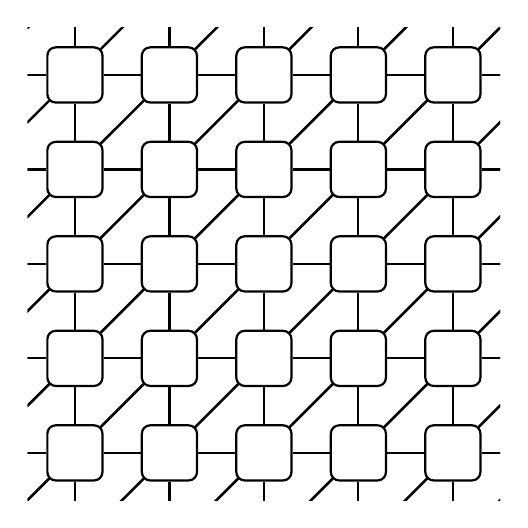
\begin{tikzpicture}[thick]
	
	\def\width{5}
	\def\height{5}
	
	% Space between node centers
	\def\spacescale{1.2}
	
	% Rounding on edges of chips
	\def\rounding{0.7ex}
	
	\pgfmathtruncatemacro{\widthh}{\width-1}
	\pgfmathtruncatemacro{\heightt}{\height-1}
	
	\tikzset{
		chip/.style={draw,rounded corners=\rounding,minimum size=0.7cm}
	}
	
	% Clip off the extra row of chips around the edge that are added to ensure we
	% end up with lots of wires dangling off the edge.
	\clip (-0.5*\spacescale,-0.5*\spacescale) rectangle
	      (\spacescale*\width-0.5*\spacescale,
	       \spacescale*\height-0.5*\spacescale);
	
	% The chips
	\foreach \x in {-1,...,\width}{
		\foreach \y in {-1,...,\height}{
			\node [chip] (chip X\x Y\y) at (\spacescale*\x, \spacescale*\y) {};
		}
	}
	
	% Edge links...
	\tikzset{
		edge wire/.style={}
	}
	
	% The wires
	\foreach \x in {0,...,\width}{
		\foreach \y in {0,...,\height}{
			\pgfmathtruncatemacro{\xx}{\x-1}
			\pgfmathtruncatemacro{\yy}{\y-1}
			
			% South-West to North-East
			\ifthenelse{\xx < 0 \OR \xx = \widthh \OR \yy < 0 \OR \yy = \heightt}{
				\draw [shorten >=-0.5*\rounding,shorten <=-0.5*\rounding]
				      [edge wire]
				      (chip X\x Y\y) to (chip X\xx Y\yy);
			}{
				\draw [shorten >=-0.5*\rounding,shorten <=-0.5*\rounding]
				      (chip X\x Y\y) to (chip X\xx Y\yy);
			}
				
				% South to North
			\ifthenelse{\yy < 0 \OR \yy = \heightt}{
				\draw [edge wire]
				      (chip X\x Y\y) to (chip X\x Y\yy);
			}{
				\draw (chip X\x Y\y) to (chip X\x Y\yy);
			}
				
				% West to East
			\ifthenelse{\xx < 0 \OR \xx = \widthh}{
				\draw [edge wire]
				      (chip X\x Y\y) to (chip X\xx Y\y);
			}{
				\draw (chip X\x Y\y) to (chip X\xx Y\y);
			}
		}
	}
	
\end{tikzpicture}

					\caption{Connections between chips (dots) with wrap-around
					connections not shown}
					\label{fig:spinnaker-chips}
				\end{subfigure}
				
				\caption{Overview of the SpiNNaker architecture.}
				\label{fig:spinnaker-architecture}
			\end{figure}
		
		\subsection{Routing}
			
			The on-chip router is table-based meaning that routing decisions are taken
			based on a set of predetermined choices loaded into a memory before
			simulations begin. The router operates on individual packets of data which
			are either 40 or 72 bits in length. These packets are short compared with
			those commonly used in super-computers which can be several kilobytes
			long.  Such networks are typically designed to transfer larger blocks of
			data, possibly many kilobytes long. SpiNNaker, however, is designed to
			primarily deal with SNNs where only the spikes' existence needs to be
			transmitted requiring little or no associated data.  The system supports
			four different kinds of packet:
			
			\begin{description}
				
				\item[Point-to-Point (P2P)] Addressed to an individual chip and will be
				passed to the core arbitrarily selected by the chip as the `monitor'
				core. Packets are routed using a table.
				
				\item[Multicast (MC)] Sent by a single core and delivered to a
				predetermined set of cores in the system. Packets are routed according
				to their source address and do not explicitly store the destination
				cores. Packets are routed using tables.
				
				\item[Fixed Route (FR)] Automatically routed to a predefined central
				point in the system. Used, for example, to collect diagnostic
				information back to the host machine. By not requiring an address a
				larger payload can be attached.
				
				\item[Nearest Neighbour (NN)] Routed to one or all of the immediate
				neighbours of a chip without the need for a routing table. On system
				start up routing tables have not been initialised and so NN packets are
				used to initially load the tables.
				
			\end{description}
			
			\subsubsection{Routing Scheme}
				
				Table based routing allows a wide array of possible routing schemes to
				be implemented conditional to two key constraints. First, the route
				taken by a packet with a particular source/destination address will
				always take the same path through the system. This is known as
				deterministic oblivious routing as the scheme is unaware of the system's
				state and cannot react to load imbalance. It is worth noting that
				schemes still exist which can improve load balance in the general case
				\cite{singh02}.
				
				\begin{figure}
					\center
					\input{figures/dimension-order-routing}
					\caption[Dimension order routing in SpiNNaker.]{Dimension order routing
					in SpiNNaker showing a path from node $S$ to $T$.}
					\label{fig:dimension-order-routing}
				\end{figure}
				
				Current versions of the routing software use simple dimension order
				routing. Here, the three axes along which packets can travel are
				considered to be three `dimensions'\footnote{The three dimensions in
				SpiNNaker's toroid are not orthogonal as would be the case in a
				conventional torus network. This is the cause of some of the slightly
				unintuitive properties of the topology.}. Packets travel along a given
				dimension until they can get no closer at which point they move onto the
				next dimension as shown in figure \ref{fig:dimension-order-routing}.
				Such paths are easily computed as shown in \cite{nocetti02} and are
				minimal in the number of hops required.
			
			\subsubsection{Multicast}
				
				Multicast packets allow SpiNNaker to handle the efficient distribution
				of spikes from heavily connected neurons in the system without requiring
				a unique packet to be sent to each destination. Instead a single packet
				is transmitted which is able to `fork' to reach multiple processors
				later in its journey.
				
				Unlike P2P packets, for which the route for every possible chip address
				(16 bits) can be stored in a routing table of around 25 kilobytes, MC
				packets are routed based on a 32 bit key which uniquely identifies the
				neuron which fired.  Exhaustively storing the route for every possible
				32-bit key is not possible since 24 bits are required for each entry
				thus requiring a 12 gigabyte routing table.
				
				Instead of an exhaustive table, one with 1,024 entries is used. The
				router looks up the 32-bit key of MC packets and, if a matching entry
				exists, uses that entry to decide where to route the packet. If no entry
				exists, the packet is forwarded to the link physically opposite the one
				through which it entered. As a result, the routing table only requires
				an entry at the entry point into the network, where the packet changes
				direction and where it is to be delivered to a core.
				
				Since the route for messages with a given key will only pass through or
				change direction in a small number of places, most routers in the system
				won't need to include an entry in their routing table. As a result this
				small size of routing table is hoped to be adequate.
				
				\begin{figure}[t!]
					\begin{subfigure}[b]{0.24\textwidth}
						\center
						\input{figures/multicast-routing-a}
						\caption{}
						\label{fig:multicast-routing-a}
					\end{subfigure}
					\begin{subfigure}[b]{0.24\textwidth}
						\center
						\input{figures/multicast-routing-b}
						\caption{}
						\label{fig:multicast-routing-b}
					\end{subfigure}
					\begin{subfigure}[b]{0.24\textwidth}
						\center
						\input{figures/multicast-routing-c}
						\caption{}
						\label{fig:multicast-routing-c}
					\end{subfigure}
					\begin{subfigure}[b]{0.24\textwidth}
						\center
						\input{figures/multicast-routing-d}
						\caption{}
						\label{fig:multicast-routing-d}
					\end{subfigure}
					
					\center
					\begin{tabular}{c c c c c}
						\toprule
							Route & Router Entries & Total Hops & Hops to $T_1$ & Hops to $T_2$ \\
						\midrule
							(a)   & 4              & 5          & 3             & 2             \\
							(b)   & 5              & 4          & 4             & 2             \\
							(c)   & 4              & 4          & 3             & 3             \\
							(d)   & 4              & 4          & 3             & 2             \\
						\bottomrule
					\end{tabular}
					
					\caption[Multicast routing examples.]{Multicast routing examples from
					$S$ to $T_1$ and $T_2$.}
					\label{fig:multicast-routing}
				\end{figure}
				
				In multicast routing, the choice of where a route should fork can have a
				great impact on system load, packet latency and routing table entry
				usage. Figure \ref{fig:multicast-routing} shows several examples of
				valid multicast routes which fork at different points, each with
				differing trade-offs.
				
				As well as guaranteeing short paths and that no routing table requires
				more than 1,024 entries, the multicast routing scheme chosen must
				attempt to ensure an even load-balance by avoiding over-using certain
				links. Various heuristic approaches based on extensions to Lee's
				algorithm have been proposed for future versions of the routing
				software\cite{davidson13}.
		
		\subsection{Hardware Abstractions}
			
			The largest SpiNNaker system is planned to contain 1,036,800 cores spread
			over 57,600 chips.  These chips are split up on 1,200 circuit boards of
			48 chips each as shown in figure \ref{fig:spinn4labelled}.
			
			\begin{figure}[p!]
				\center
				\begin{tikzpicture}[thick]
	
	\node[anchor=south west,inner sep=0] at (0,0) (image)
		{\includegraphics[width=0.5\textwidth]{figures/spinn4.png}};
	
	\begin{scope}[x={(image.south east)},y={(image.north west)}]
		%% Help with drawing
		%\draw[help lines,xstep=.1,ystep=.1] (0,0) grid (1,1);
		%\foreach \x in {0,1,...,9} { \node [anchor=north] at (\x/10,0) {0.\x}; }
		%\foreach \y in {0,1,...,9} { \node [anchor=east] at (0,\y/10) {0.\y}; }
		
		\draw [decorate,decoration={brace,raise=1ex,amplitude=1ex}]
		      (0.02,0.5) -- coordinate (left-label) (0.02,1.0);
		\node [left=1em of left-label,text width=3.5cm,align=center]
		      {High-Speed Links\\(Board-to-Board)};
		
		\draw [decorate,decoration={brace,raise=1ex,amplitude=1ex}]
		      (0.97,1.0) -- coordinate (right-label) (0.97,0.5);
		\node [right=1em of right-label,text width=3.5cm,align=center]
		      {High-Speed Links\\(Other I/O)};
		
		\draw [decorate,decoration={brace,raise=1ex,amplitude=1ex}]
		      (1.0,0.23) -- coordinate (power-label) (1.0,0.02);
		\node [right=1em of power-label] {Power Connector};
		
		\draw [decorate,decoration={brace,raise=1ex,amplitude=1ex}]
		      (0.0,0.08) -- coordinate (eth-label) (0.0,0.22);
		\node [left=1em of eth-label] {Ethernet};
	\end{scope}
	
\end{tikzpicture}

				\caption{48-chip SpiNNaker circuit board.}
				\label{fig:spinn4labelled}
			\end{figure}
			
			Each board is equipped with a number of high-speed links, six of which are
			used to connect the board's chips to their neighbours on other boards. The
			other links are reserved for connecting other I/O such as silicon retinas
			and robotic platforms \cite{davies10}. An Ethernet connection is also
			present to provide a simple, low-bandwidth link to an external host
			system.
			
			\begin{figure}[p!]
				\center
				\includegraphics[width=0.5\textwidth]{figures/spiNNaker103.jpg}
				\caption{Partially populated rack of SpiNNaker boards.}
				\label{fig:spiNNaker103}
			\end{figure}
			
			Groups of twenty-four boards are then placed in racks such as in figure
			\ref{fig:spiNNaker103} which are in turn placed, five-high, into ten
			cabinets to complete the largest planned machine. Further details of this
			arrangement are given later in
			\S\ref{sec:wiring-up-large-spinnaker-machines} where preliminary work on
			wiring schemes for the machine are described.
		
		\subsection{Connecting Boards Together}
			
			Logically, the chips on each circuit board are laid out as shown in figure
			\ref{fig:chipsOnBoard}. Touching edges represent chip-to-chip connections
			which uses a delay insensitive, parallel `2-of-7' communications scheme
			similar to that used in the on-chip network requiring 16 wires per link.
			If this technology was used to connect boards together 768 wires would be
			required.  This would be prohibitively expensive requiring highly
			specialised cables and connectors. Instead, an alternative technology,
			known as high-speed serial, is used which replaces the 768 wires with only
			24 which can be carried by cheap, commodity cables. This technology allows
			eight board-to-board connections to share a single cable grouped as shown in
			the figure.
			
			\begin{figure}
				\center
				\input{figures/chipsOnBoard}
				\caption{Logical arrangement of chips on a circuit board.}
				\label{fig:chipsOnBoard}
			\end{figure}
			
			To construct a toroid, at least three boards must be combined as shown in
			figure \ref{fig:threeboard} (an arrangement known as a threeboard).
			Figure \ref{fig:threeboardSliced} shows how the threeboard arrangement can
			be turned into a sheet which in turn can be turned into a toroid as shown
			earlier in figure \ref{fig:forming-a-torus}.
			
			\begin{figure}
				\begin{subfigure}[b]{0.45\textwidth}
					\center
					\input{figures/threeboard}
					\caption{Threeboard}
					\label{fig:threeboard}
				\end{subfigure}
				\begin{subfigure}[b]{0.45\textwidth}
					\center
					\input{figures/threeboardSliced}
					\caption{Sliced into a sheet}
					\label{fig:threeboardSliced}
				\end{subfigure}
				
				\caption[A `threeboard'.]{A `threeboard', the minimal configuration of
				boards yielding a toroid.}
			\end{figure}
			
			Arbitrarily large systems can be produced by repeating the threeboard
			pattern to create larger toroids.
	
	\break
	\section{High-Speed Serial}
		
		\label{sec:high-speed-serial}
		
		High-speed serial is the general name for a technology which allows
		high-bandwidth links to be constructed using only a few electrical wires.
		These links are the basis of many widely used technologies ranging from
		S-ATA, used for attaching consumer-grade hard disks to computers
		\cite{sataio}, to the InfiniBand interconnect designed for super-computers
		\cite{infinibandta}.
		
		Compared to older technologies such as simple parallel buses, high-speed
		serial links require more complex hardware to implement and so tend to be
		reserved for off-chip connections. They are the basis of many current Top500
		super-computer interconnects as well as SpiNNaker's board-to-board links.
		
		Traditionally, signals between components in a system have been carried by a
		set of parallel wires. Each wire carried a single bit allowing multiple bits
		to be transmitted at once. Figure \ref{fig:parallel-example-no-skew} shows
		eight parallel signals being used to transmit a message. The electrical
		signal being sent down each wire is sampled at the tick of a clock (the
		vertical lines in the figure) and the eight bits are interpreted as an ASCII
		character.
		
		In practice each of the wires carrying the parallel signal will have
		differing electrical properties due to imperfections during manufacturing
		such as slight variations in length. These differences result in the
		signals taking different times to travel along the wires, an effect known
		as skew. For a long time the skew remained insignificant compared to the
		period of the parallel signal.  As clock speeds increased, however, skew
		started to become significant enough to cause some of the parallel signals
		to arrive so far apart relative to the clock that some would be
		incorrectly sampled by the receiver resulting in transmission errors such
		as in figure \ref{fig:parallel-example-skew}.
		
		\begin{figure}
			\begin{subfigure}[b]{0.49\textwidth}
				\center
				\input{|"python2 figures/parallel_comms.py 'Hello, World!' 1.0 1.3 0"}
				\caption{No skew}
				\label{fig:parallel-example-no-skew}
			\end{subfigure}
			\begin{subfigure}[b]{0.49\textwidth}
				\center
				\input{|"python2 figures/parallel_comms.py 'Hello, World!' 1.0 1.3 0.7"}
				\caption{With skew}
				\label{fig:parallel-example-skew}
			\end{subfigure}
			
			\caption{Parallel signalling example.}
			\label{fig:parallel-example}
		\end{figure}
		
		Since wiring technology has been unable to improve fast enough to keep
		skew acceptably small for all but the shortest connections, parallel
		signalling has been replaced with high-speed serial signalling.  Here,
		bits are sent one after another as shown in figure
		\ref{fig:serial-example}. Because there is only one signal, the problem of
		skew is eliminated.
		
		\begin{figure}
			\center
			\begin{tikzpicture}
				\input{|"python2 figures/serial_comms.py '' 'Hello, World!' 1 0 0 0 0 0.4 0.2"}
			\end{tikzpicture}
			
			\caption{Serial signalling example.}
			\label{fig:serial-example}
		\end{figure}
